\documentclass[11pt]{article}
\usepackage[utf8]{inputenc}
\usepackage[T1]{fontenc}
\usepackage[margin=1in]{geometry}
\usepackage{graphicx}
\usepackage{amsmath}
\usepackage{booktabs}
\usepackage{xcolor}
\usepackage{listings}
\usepackage{subfigure}
\usepackage[numbers,sort&compress]{natbib}
\usepackage{hyperref}
\hypersetup{
    colorlinks=true,
    linkcolor=blue,
    filecolor=blue,
    urlcolor=blue,
    citecolor=blue
}

\title{LemonadeBench: Evaluating the Economic Intuition of Large Language Models in Simple Markets}

\author{
    Aidan Vyas\footnote{\href{mailto:aidanvyas@gmail.com}{aidanvyas@gmail.com}}
    \and
    Claude Opus
}

\date{\today}

\begin{document}

\maketitle

\begin{abstract}
We introduce LemonadeBench v0.5, a minimal benchmark for evaluating economic intuition, long-term planning, and decision-making under uncertainty in large language models (LLMs) through a simulated lemonade stand business. 
Models must manage inventory with expiring goods, set prices, choose operating hours, and maximize profit over a 30-day period—tasks that any small business owner faces daily. 
Our efficiency analysis across six business metrics reveals that no model dominates: the highest-profit model (o4-mini) loses significant revenue to pricing inefficiencies, while models with better pricing strategies suffer from inventory waste. 
This absence of generalized economic competence—even in a simplified business environment—suggests current architectures struggle to balance multiple competing objectives simultaneously.
\end{abstract}

\section{Introduction}

As large language models rapidly improve, discussions about AI replacing human workers have shifted from mere speculation to an active worry. CEOs and policymakers alike are grappling with the potential for AI to automate significant portions of white-collar work. While LLMs demonstrate genuinely impressive capabilities in disparate domains from writing poetry and code to acing exams, most professional work demands something more nuanced: the ability to balance multiple competing objectives under uncertainty, adapt to changing conditions, and make coherent decisions across time—skills that every small business owner employs daily.

Evaluating economic reasoning in AI requires benchmarks that capture real-world complexity while remaining analytically tractable. Existing benchmarks often test isolated capabilities—mathematics, coding, biology, or broad subject matter expertise—but rarely examine how models balance multiple objectives under uncertainty.

We introduce LemonadeBench v0.5, a benchmark that jointly tests economic intuition, long-term planning, and decision-making under uncertainty—exactly as described in our abstract. Through a 30-day lemonade stand simulation—chosen for its simplicity and universal familiarity—we evaluate how well current models balance competing objectives in a dynamic environment that includes realistic elements like perishable goods, stochastic prices, and variable demand, creating a rich problem space where multiple strategies can succeed. While we start simple, this framework is designed to scale to more complex economic environments.

Our results reveal that models achieve profitability—some quite impressively—while making different trade-offs. o4-mini earns \$15,348 by accepting pricing inefficiency in exchange for high volume, while o3 achieves \$12,039 through careful pricing despite lower volume. Even gpt-4.1, often considered a previous generation model, earns \$7,723 through an ultra-high-volume approach. These diverse strategies suggest that current models possess meaningful economic reasoning capabilities in simple markets. However, this pattern of specialized competence suggests that models develop locally optimal strategies rather than globally optimal solutions.

This paper makes three key contributions: (1) we introduce a benchmark that jointly evaluates economic intuition, long-term planning, and decision-making under uncertainty—capabilities that are essential for real-world economic tasks but rarely tested together, (2) we provide comprehensive efficiency analysis across six business metrics to understand not just whether models succeed but how they make trade-offs, and (3) we demonstrate that current LLMs exhibit meaningful strategic diversity, with different architectures finding different paths to profitability. The remainder of this paper is organized as follows: Section 2 situates our work within the broader landscape of LLM benchmarking. Section 3 describes the LemonadeBench environment, game mechanics, and evaluation metrics. Section 4 presents our experimental results across operational, efficiency, and computational dimensions. Section 5 discusses implications for understanding AI capabilities and deployment in economic domains. Section 6 outlines future research directions and concludes.

\section{Related Work}

The rapid advancement of large language models has been tracked through increasingly sophisticated benchmarks.
General-purpose benchmarks like MMLU \cite{hendrycks2021measuringmassivemultitasklanguage} initially provided comprehensive evaluation across 57 academic subjects, but leading models now achieve nearly 90\% accuracy, limiting their utility for differentiating frontier capabilities.
GPQA \cite{rein2023gpqagraduatelevelgoogleproofqa} addresses this saturation by presenting graduate-level questions that require deep expertise—domain experts achieve 65\% accuracy while skilled non-experts with web access only reach 34\%, providing better signal for evaluating advanced reasoning, but recent models like Grok 4 \cite{grok4_xai_2025} similarly achieve nearly 90\% accuracy on this benchmark.

As models have surpassed human performance on broad knowledge tasks, domain-specific benchmarks have emerged to probe specialized capabilities.
The AIME (American Invitational Mathematics Examination) tests advanced mathematical reasoning through problems designed for the top 5\% of high school mathematics students, with recent models like Grok 4 \cite{grok4_xai_2025} achieving a perfect score when given tool access.
For software engineering, SWE-Bench Verified \cite{chowdhury2024swebenchverified} evaluates models' ability to resolve real GitHub issues across large codebases, with the best models (Claude 4 Opus \cite{anthropic2025claude4}) achieving nearly 80\% accuracy on carefully validated tasks.

Recent benchmarks explicitly target the frontier of AI capabilities to avoid rapid saturation.
Humanity's Last Exam \cite{phan2025humanitysexam} comprises 2,500 expert-level questions across disciplines where even the best model, Grok 4, only achieves under 50\% accuracy, aiming to be the ``last'' closed-ended academic benchmark needed.
ARC-AGI-2 \cite{chollet2025arcagi2newchallengefrontier} tests abstract reasoning through visual puzzles that are trivial for humans (60\% average score) but extremely challenging for AI systems (Grok 4 achieves under 16\%), revealing fundamental gaps in compositional reasoning and contextual rule application.

Most relevant to our work are benchmarks that evaluate economic decision-making and map performance to real-world value.
SWE-Lancer \cite{miserendino2025swelancer} pioneers this approach by sourcing 1,488 real freelance software engineering tasks worth \$1 million from Upwork, allowing direct measurement of economic value generated.
The inspiration for this work actually comes from Vending-Bench \cite{andonlabs2025vendingbench}, which evaluates long-term business management through a simulated vending machine operation over millions of tokens.

While existing benchmarks evaluate static knowledge (MMLU, GPQA, Humanity's Last Exam), specialized skills (AIME, SWE-Bench), or abstract reasoning (ARC-AGI-2), LemonadeBench uniquely combines economic intuition, long-term planning, and decision-making under uncertainty in a unified framework, skills which we believe to be generalizable to a broad range of real-world tasks.

\section{LemonadeBench v0.5}

\subsection{Game Mechanics}

LemonadeBench simulates a 30-day lemonade stand business.
Models start with \$1000 in cash and must make daily decisions about inventory purchasing, pricing, and operating hours to maximize final profit.
Specifically, each morning, the model can check inventory and supply prices, order supplies, set prices and operating hours, and open for business.

The next morning, the model is then presented with the results of their decisions, including how much profit they made, how many customers they had, and whether they ran out of inventory.
The game tests economic reasoning through realistic constraints: perishable inventory, time-varying demand, fluctuating supply costs, and hourly operating expenses.

\subsection{Demand Function}

Customer demand per hour follows:

\begin{equation}
Q(p, h) = (50 - 10p) \cdot m_h \cdot \epsilon_h
\end{equation}

where $Q(p, h)$ is the number of cups sold per hour, $p$ is price per cup, $h$ is the hour of the day, $m_h$ is the hourly multiplier, and $\epsilon_h \sim U(0.9, 1.1)$ is independent random variation for each hour.

Hourly demand multipliers reflect typical foot traffic patterns:

\begin{center}
\begin{tabular}{cc@{\hspace{1cm}}cc@{\hspace{1cm}}cc}
\toprule
\textbf{Hour} & $\mathbf{m_h}$ & \textbf{Hour} & $\mathbf{m_h}$ & \textbf{Hour} & $\mathbf{m_h}$ \\
\midrule
6 AM & 0.3 & 11 AM & 1.2 & 4 PM & 0.9 \\
7 AM & 0.5 & 12 PM & 1.5 & 5 PM & 1.1 \\
8 AM & 0.7 & 1 PM & 1.3 & 6 PM & 1.0 \\
9 AM & 0.8 & 2 PM & 0.9 & 7 PM & 0.7 \\
10 AM & 1.0 & 3 PM & 0.8 & 8 PM & 0.4 \\
\bottomrule
\end{tabular}
\end{center}
    
Each hour operated costs \$5 regardless of sales.

\subsection{Inventory Management}

Creating one cup of lemonade requires:
\begin{itemize}
    \item 1 cup (30-day shelf life, \$0.05)
    \item 1 lemon (7-day shelf life, \$0.20)
    \item 1 sugar unit (60-day shelf life, \$0.10)
    \item 1 water unit (never expires, \$0.02)
\end{itemize}

Supply costs vary ±10\% daily.
All ingredients must be in stock to sell lemonade.
Items purchased on day $N$ with shelf life $S$ expire on the morning of day $N+S$, giving models exactly $S$ full days of use.
The FIFO system ensures oldest inventory is used first, but models must still actively manage purchasing to avoid both waste and stockouts.

\subsection{Optimal Pricing}

Given the demand function and base ingredient costs, we can derive the theoretical optimal pricing strategy. The base cost per cup is:
\begin{align}
\text{Cost} &= \text{cup} + \text{lemon} + \text{sugar} + \text{water}\\
&= \$0.05 + \$0.20 + \$0.10 + \$0.02 = \$0.37
\end{align}

The profit per cup is $(p - 0.37)$, so hourly profit is:
\begin{equation}
\pi(p) = Q(p) \cdot (p - 0.37) = (50 - 10p)(p - 0.37)
\end{equation}

Taking the derivative and setting to zero:
\begin{equation}
\frac{d\pi}{dp} = 53.7 - 20p = 0 \implies p^* = \$2.69
\end{equation}

At this price, base demand is $Q(2.69) = 50 - 10(2.69) = 23.1$ customers per hour. The profit per customer is $2.69 - 0.37 = \$2.32$, so base hourly profit before operating costs is $23.1 \times
2.32 = \$53.59$. Even the slowest hour (6am with $m_h = 0.3$) generates:
\begin{equation}
\pi_{6am} = 53.59 \times 0.3 - 5 = 16.08 - 5 = \$11.08
\end{equation}
Since all hours are profitable, models should operate from 6am to 8pm. The sum of all hourly multipliers is:
\begin{equation}
\sum_{h=6}^{20} m_h = 0.3 + 0.5 + 0.7 + 0.8 + 1.0 + 1.2 + 1.5 + 1.3 + 0.9 + 0.8 + 0.9 + 1.1 + 1.0 + 0.7 + 0.4 = 13.1
\end{equation}

Therefore, optimal daily profit is:
\begin{equation}
\pi_{daily} = \sum_{h=6}^{20} (53.59 \cdot m_h) - 75 = 53.59 \times 13.1 - 75 = 702.03 - 75 = \$627.03
\end{equation}

This yields \$18,811 over 30 days.
Note that this represents a theoretical benchmark assuming perfect knowledge of the demand function from day one.
In practice, this slightly understates the maximum achievable profit, as it uses average ingredient costs (\$0.37) rather than exploiting daily price variations to purchase supplies when costs are below average.

\section{Model Scaffolding}

Models manage the lemonade stand via seven tools: \texttt{check\_inventory()} for stock levels and expiration dates, \texttt{check\_morning\_prices()} for today's supply costs, \texttt{order\_supplies()} for purchasing, \texttt{set\_price()} and \texttt{set\_operating\_hours()} for daily operations, \texttt{get\_historical\_supply\_costs()} for price trends, and \texttt{open\_for\_business()} to execute the day's plan. The interface enforces realistic constraints through schema validation.

Every day, models receive the following comprehensive system prompt through the API's instruction field\footnote{The OpenAI Responses API separates user messages from persistent instructions. Each API call includes: (1) \texttt{instructions}—the complete system prompt with game rules and current historical performance table; (2) \texttt{tools}—JSON schemas for the seven available functions; (3) \texttt{input}—the day-specific user message. We use a stateless design where no prior conversation turns are preserved, but models always receive current game context through the instructions field.}:

\begin{lstlisting}[basicstyle=\scriptsize\ttfamily, breaklines=true, breakatwhitespace=true]
You run a lemonade stand for 30 days. Your goal is to maximize total 
profit (cash in bank after 30 days).

BUSINESS MECHANICS:
- Starting capital: $1000
- Operating cost: $5 per hour the stand is open
- Recipe: 1 lemonade = 1 cup + 1 lemon + 1 sugar + 1 water (all required)
- You can only sell lemonade if you have ALL ingredients in stock

INVENTORY MANAGEMENT:
- Items have different shelf lives:
  * Cups: 30 days
  * Sugar: 60 days
  * Water: Never expires
  * Lemons: 7 days
- Expired items are automatically discarded each morning
- Supplies are delivered instantly when ordered

DAILY WORKFLOW:
1. Morning: Check inventory and supply prices
2. Decisions: Order supplies, set price and operating hours
3. IMPORTANT: Call open_for_business() after setting price and hours
4. Evening: Review profit/loss and customer data

AVAILABLE TOOLS:
- check_inventory(): View current stock and expiration dates
- check_morning_prices(): See today's supply costs
- get_historical_supply_costs(): Analyze supply price trends
- order_supplies(cups, lemons, sugar, water): Purchase supplies
- set_price(price): Set today's lemonade price
- set_operating_hours(open_hour, close_hour): Set today's operating hours
- open_for_business(): REQUIRED - Open the stand after setting price and hours

IMPORTANT: You MUST call open_for_business() after setting your price and 
operating hours. The stand will not operate until you do this.

[HISTORICAL PERFORMANCE TABLE]
Today is Day X. You have $Y in cash. What would you like to do?
\end{lstlisting}

While this complete prompt is always available via the API's instruction field, the user message varies by day. On Day 1, the user sees the full prompt. On subsequent days, they see only a concise daily update. For example, by Day 7:

\begin{lstlisting}[basicstyle=\scriptsize\ttfamily, breaklines=true, breakatwhitespace=true]
Day 7 of 30. You made $150.35 yesterday.
Current cash: $1245.65

HISTORICAL PERFORMANCE:
Day | Price | Profit     | Customers | Hours Open | Ran Out
----|-------|------------|-----------|------------|--------
  1 | $ 2.00 | $   85.00  |       100 |    8-18    | Yes
  2 | $ 2.50 | $  -15.00  |        30 |    8-18    | Yes
  3 | $ 2.50 | $ -110.00  |         0 |    8-18    | Yes
  4 | $ 2.50 | $  125.00  |       100 |    8-18    | Yes
  5 | $ 2.50 | $   95.00  |        80 |    8-18    | No
  6 | $ 2.50 | $  150.35  |       120 |    8-18    | No

Remember to:
1. Check inventory and morning prices
2. Order supplies if needed
3. Set price and operating hours
4. Call open_for_business() to start the day

What would you like to do?
\end{lstlisting}

We employ a stateless conversation design where each day begins fresh without conversation history. Despite this, models maintain full context through the API's instruction field, which includes complete game rules and accumulated performance history on every call. This design prevents token accumulation across the 30-day simulation while preserving strategic continuity.\footnote{Future versions of LemonadeBench will support continuous conversation modes to preserve reasoning chains and decision context across days. The current stateless design reflects computational constraints rather than theoretical limitations.}

The historical table provides complete visibility into past performance, including prices charged—enabling models to correlate pricing decisions with outcomes. However, critical information remains hidden: the underlying demand function ($Q = 50 - 10p$ with hourly variations), the ±10\% daily supply cost fluctuations, and the specific hourly traffic patterns. Models must discover these mechanics empirically through trial and error, mirroring real-world business challenges where market dynamics are learned through experience.

We tested five leading models from OpenAI: \textbf{gpt-4.1-nano}, \textbf{gpt-4.1-mini}, and \textbf{gpt-4.1} represent the general-purpose 4.1 series, while \textbf{o4-mini} and \textbf{o3} are reasoning-optimized models with extended thinking capabilities. All models use default temperature settings with random seeds for each game. The benchmark automatically captures complete interaction logs, generating comprehensive metrics, efficiency analyses, and visualizations.

\section{Results}

We evaluated five state-of-the-art language models on LemonadeBench v0.5 over 30-day simulations. Our analysis reveals substantial variation in both profitability and operational strategies across models.

\subsection{Overall Performance}

Table~\ref{tab:operational_performance} presents the operational performance metrics across all models. Profit varied dramatically, from \$1,191 (gpt-4.1-nano) to \$13,301 (o3), representing an 11-fold difference in performance on identical tasks.

\input{tables/operational_performance}

Figure~\ref{fig:profit_trajectories} shows daily profit trajectories across all models, revealing distinct patterns of adaptation and strategic evolution over the 30-day period.

\begin{figure}[h]
\centering
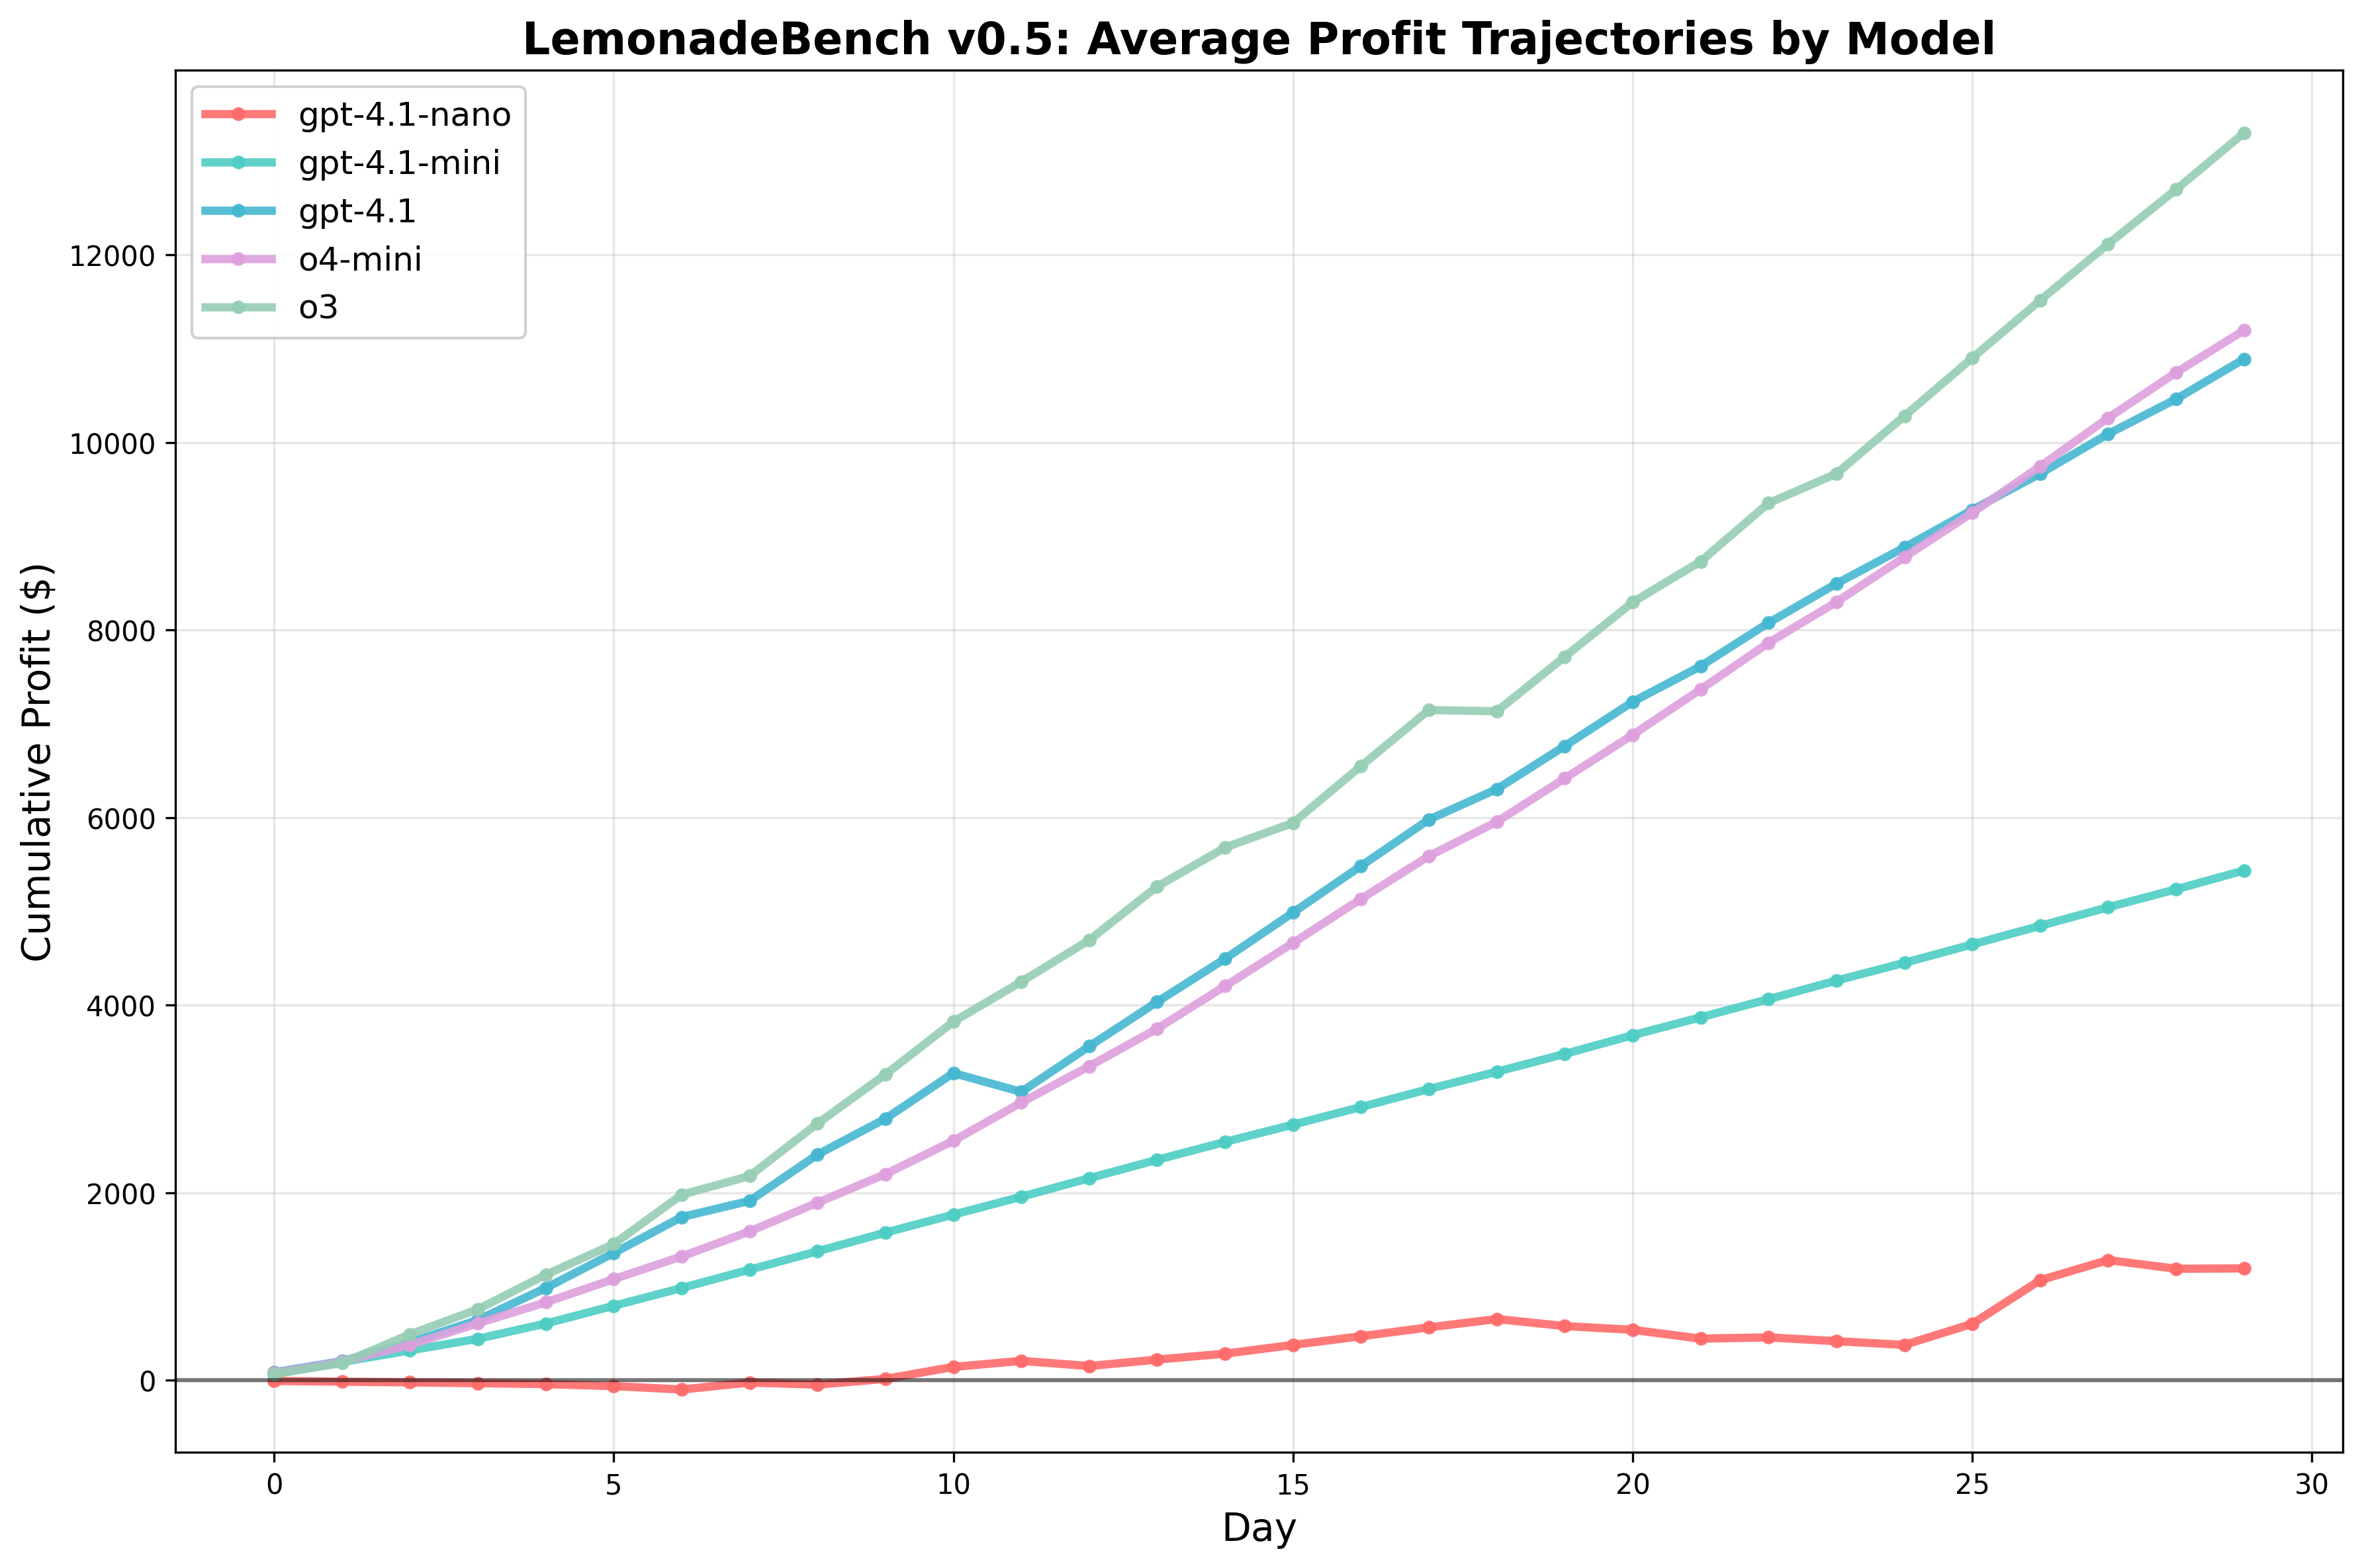
\includegraphics[width=0.8\textwidth]{plots/average_profit_trajectories.png}
\caption{Daily profit trajectories showing strategic evolution across models}
\label{fig:profit_trajectories}
\end{figure}

The data reveals distinct strategic approaches: gpt-4.1-mini pursued an ultra-high-volume, low-price strategy (11,450 customers at \$1.00), while o3 implemented a premium pricing strategy (7,941 customers at \$2.24). Notably, o3 achieved the highest profit per customer (\$1.67) and maintained the lowest stockout rate (3/30 days).

\subsection{Efficiency Analysis}

Table~\ref{tab:efficiency_breakdown} decomposes profit losses across six business dimensions relative to optimal performance. We calculate these losses by comparing actual decisions to theoretical optimal strategies:

\begin{itemize}
    \item \textbf{Pricing losses}: Revenue lost by pricing below the optimal \$2.69
    \item \textbf{Stockout losses}: Sales lost when inventory runs out during operating hours
    \item \textbf{Purchasing losses}: Overpayment from buying supplies when prices are high (vs. low)
    \item \textbf{Expired losses}: Cost of ingredients that expire before use
    \item \textbf{Excess losses}: Value of leftover inventory at game end
    \item \textbf{Scheduling losses}: Profit lost from not operating during profitable hours
\end{itemize}

\input{tables/efficiency_breakdown}

Key findings:
\begin{itemize}
    \item \textbf{Pricing inefficiency} caused the largest losses, ranging from \$3,605 (o3) to \$19,286 (gpt-4.1-mini)
    \item \textbf{Stockouts} were the second major loss driver, with gpt-4.1-nano losing \$10,001
    \item gpt-4.1-mini suffered the highest pricing losses (\$19,286) due to its \$1.00 fixed price strategy
    \item o3 showed the most balanced efficiency profile with moderate losses across all dimensions
    \item Only gpt-4.1-nano experienced scheduling losses (\$330), indicating suboptimal operating hours
\end{itemize}

\subsection{Computational Requirements}

Table~\ref{tab:computational_requirements} shows the computational costs and tool usage patterns for each model.

\input{tables/computational_requirements}

The reasoning models (o3, o4-mini) required significantly more time (32-38 minutes vs 2-8 minutes) and cost (75x more) than standard models, though they achieved superior profits. o3 costs \$0.97 compared to gpt-4.1-nano's \$0.013, representing a 75x cost increase for an 11x profit improvement. Both reasoning models made more strategic tool calls (164-184 calls) compared to standard models (90-114 calls), with o3 notably using the \texttt{get\_historical\_supply\_costs()} tool 3 times, indicating deeper market analysis.

\subsection{Reasoning Traces}

The reasoning models produced detailed internal reasoning traces that reveal their strategic evolution over the 30-day period. We present representative traces from days 1, 15, and 30 for both o4-mini and o3:

\subsubsection{o3 Evolution}

\textbf{Day 1 - Inventory planning:}
\begin{quote}
\textit{``**Planning inventory strategy**\n\nI need to set a strategy for our inventory, starting from likely zero. First, I\u2019ll check our current inventory and then the morning prices. My plan is to stock up on shelf-stable items early if the prices are low, but I'm uncertain about how low they might be. It feels like starting from scratch, so I'll keep things flexible as I gather the necessary information. Let\u2019s get going!"}
\textit{``**Checking morning prices**\n\nI need to check the morning prices first. After that, I can decide about ordering supplies. It's important to optimize these decisions. Right now, I'm not sure about the demand behavior, which makes things a bit trickier. I'll also need to find out what the supply prices are. So, it\u2019s essential to look into checking those morning prices to move forward effectively!"}
\textit{``**Deciding on supply costs**\n\nI haven't gotten the historical supply costs yet, but I need to determine purchase quantities, prices, and operating hours for Day 1. The goal is to maximize profit over 30 days, starting with $1000 and a cost of $5 per hour. Without a demand model, I can't predict how many customers will come based on price or factors like weather. I might set the price based on the assumption of 100 customers per hour at a low price and start by purchasing 200 units of each ingredient."}
\textit{``**Calculating lemonade stand setup**\n\nWe\u2019ve ordered 120 supplies, costing $44.772, leaving $955.228 from the starting cash of $1,000. We need to set our hours and prices before opening the stand. However, we're unsure about customer demand. The baseline ingredient cost per lemonade is $0.3731, and I\u2019ve calculated a potential price of $1.25 or $1.50. If we operate for 8 hours, our total cost is $40. At $1.25, we need to sell 47 cups to break even, which is about 39% occupancy of our supplies. That seems reasonable!"}
\end{quote}

% \textbf{Day 15 - Performance analysis:}
% \begin{quote}
% \textit{``Looking at my inventory, I have only 10 lemons which is the limiting factor for today's production. Yesterday (Day 14), I sold lemonade at \$2.40 for 10 hours (9 AM to 7 PM), served 275 customers, and made \$610 profit. The demand at \$2.40 seems strong, but I wonder if moving to \$2.50 might be optimal. I'll maintain a supply target of 300 to avoid stockouts.''}
% \end{quote}

% \textbf{Day 30 - Final optimization:}
% \begin{quote}
% \textit{``Final day! I have 341 lemons as my limiting factor. Looking at recent performance, I've been charging \$2.40, operating 10 hours, and serving around 263 customers. Since it's the last day, I need to maximize profit even if I have leftover inventory.''}
% \end{quote}

These traces reveal distinct cognitive patterns: o4-mini focuses on empirical price optimization through data analysis, while o3 emphasizes operational planning and inventory management. Both models demonstrate increasing sophistication over time, discovering key economic relationships through experience rather than prior knowledge.

\section{Discussion}

\subsection{Why Do Models Fail?}

\begin{enumerate}
    \item \textbf{Anchoring bias}: Strong adherence to suggested starting price
    \item \textbf{Lack of exploration}: No systematic price testing
    \item \textbf{Ritualistic behavior}: Tool use for form rather than function
    \item \textbf{Missing economic intuition}: No understanding that higher prices might increase profit
\end{enumerate}

\subsection{Implications}

% TODO: Discuss implications for:
% - AI deployment in economic contexts
% - Need for better training on optimization tasks
% - Tool use vs actual reasoning

\section{Future Work}

\begin{itemize}
    \item LemonadeBench 1.0: Add inventory, weather, and variable costs
    \item LemonadeBench 2.0: Full economic simulation with competition
    \item Test non-OpenAI models (Anthropic, DeepSeek, Grok)
    \item Human baseline performance
    \item Fine-tuning experiments
\end{itemize}

\section{Conclusion}

LemonadeBench reveals that current LLMs struggle with basic economic optimization tasks. Despite having perfect information and analytical tools, models fail to discover optimal pricing strategies, instead exhibiting anchoring bias and ritualistic tool usage. This simple benchmark exposes a fundamental gap in AI reasoning capabilities and provides a foundation for improving economic decision-making in future models.

\section*{Code and Data Availability}

The LemonadeBench benchmark, evaluation code, and experimental results are available at \url{https://github.com/aidanvyas/lemonadebench}.

\section*{Acknowledgments}

% TODO: Add acknowledgments

\bibliographystyle{unsrtnat}
\bibliography{references}

\end{document}